\documentclass[letterpaper]{article} % DO NOT CHANGE THIS
\usepackage[submission]{aaai2027}  % DO NOT CHANGE THIS
% The serif, sans-serif, and monospaced fonts are loaded automatically by
% aaai2027.sty (newtxtext, helvet, courier). DO NOT add \usepackage{times},
% \usepackage{helvet}, \usepackage{courier}, or any other font package.
\usepackage[hyphens]{url}  % DO NOT CHANGE THIS
\usepackage{graphicx} % DO NOT CHANGE THIS
\urlstyle{rm} % DO NOT CHANGE THIS
\def\UrlFont{\rm}  % DO NOT CHANGE THIS
\usepackage{natbib}  % DO NOT CHANGE THIS AND DO NOT ADD ANY OPTIONS TO IT
\usepackage{caption} % DO NOT CHANGE THIS AND DO NOT ADD ANY OPTIONS TO IT
\frenchspacing  % DO NOT CHANGE THIS

\usepackage{amsmath,amssymb}
\usepackage{booktabs}
\newcommand{\model}{Z-Image}
\newcommand{\eg}{\emph{e.g.}}
\newcommand{\ie}{\emph{i.e.}}

% Keep the \pdfinfo as shown here. There's no need
% for you to add the /Title and /Author tags.
\pdfinfo{
/TemplateVersion (2027.1)
}

\setcounter{secnumdepth}{0} % AAAI: unnumbered sections by default

\title{Identity-Match Is Not Enough: Composition-Collapse Blind Spots in Two Cheap Reference-Conditioning Mechanisms for a Frozen Anime Diffusion Transformer}
\author{
    Anonymous Submission
}
\affiliations{
    %
}

\begin{document}

\maketitle

\begin{abstract}
Reference-conditioned identity preservation is normally bought with a
purpose-trained adapter on real-face data or a base model already
pretrained for editing; neither transfers to a frozen, pure
text-to-image (T2I) anime diffusion transformer that must remain
unmodified. We activate such a model with two cheap, independent
mechanisms -- training-free attention key/value injection from a
reference image, and a 0.06\%-parameter band-LoRA -- and show both are
competitive with a same-class trained adapter at a fraction of the cost.
The paper's central finding is methodological: identity-match rate, the
field's standard headline metric, is not merely incomplete but actively
misleading, in two mechanistically unrelated settings. First, a
training-free recipe tuned on a small development set raises raw
identity-match rate (23\%$\to$40\%) but also raises a severe
composition-collapse (collage/tiling) defect rate from 20\% to 82\%,
collapsing usable-output rate from 53\% to 15\% -- identity-match alone
would have recommended the worse recipe. Second, a pre-registered
ablation on the unrelated training-light mechanism, testing whether a
specific transformer-layer band is responsible for identity capacity,
finds identity-match statistically flat across all four tested layer
bands -- a null that replicates on a second held-out subject set. An
apparent 8.6$\times$ defect-rate gradient across the same bands,
CI-decisive on the first set, did not survive our own audit: it fails
to replicate cross-set, and a confound-free re-run of its reference arm
(matched training manifest, no generation-style prefix) erases it on
the original set, with subject-clustered CIs disjoint from the original
value. We report the full audit trail -- the failed hypothesis and the
self-refuted gradient -- as evidence that identity-match-only,
single-set, single-protocol evaluation is a systematically optimistic
basis for reference-conditioning claims.
\end{abstract}

\section{Introduction}\label{sec:intro}

Reference-conditioned identity preservation -- feed a reference portrait,
get the same character in a new scene -- is normally bought one of two
ways: train a dedicated adapter on a large paired dataset
\citep{ye2023ipadapter,li2023photomaker,wang2024instantid}, or switch to
an instruction-following edit model whose base was already pretrained
for image-to-image tasks \citep{blackforest2025fluxkontext}. Neither
route is available when the base model must remain a frozen, pure
text-to-image (T2I) diffusion transformer: no per-subject or general
fine-tuning, no departure from T2I semantics into edit-model territory,
no library modification. We show such a model -- a frozen anime T2I DiT,
Z-Image \citep{zimage2025} -- can be activated as a reference-conditioned
identity generator by two cheap, mechanistically independent
interventions: concatenating the reference image's attention key/value
tensors into a restricted band of self-attention layers at inference
time (zero training), and a rank-8 LoRA on 0.06\% of backbone parameters
within the same layer band (minutes of training, not per-subject).

Getting either mechanism to actually work exposes the same blind spot
twice. Both mechanisms have a natural, cheap-to-measure headline metric
-- does the generated character look like the reference? -- and both
times, optimizing or ablating against that metric alone would have led
to the wrong conclusion. The training-free mechanism's naive
position-preserving key injection causes literal copy-paste ``ghosting''
because the reference and target token grids share the same RoPE
coordinate origin; a frequency-gated fix removes the ghosting and *does*
raise raw identity-match rate on a small development set (23\%$\to$40\%)
-- but held-out validation with a defect-aware judge shows the same
recipe also raises a severe composition-collapse defect rate from 20\%
to 82\%, so the rate of an actually usable image collapses from 53\% to
15\%. The training-light mechanism's layer-position ablation was
pre-registered to test whether a specific 16-layer band is uniquely
responsible for identity-conditioning capacity; identity-match turns out
to be statistically flat across every tested band (95\% CI overlapping,
confirmed under subject-level clustering, and replicated on a second
held-out subject set) -- the hypothesis fails. An apparent 8.6$\times$
defect-rate gradient across the same bands then failed our own audit:
it does not replicate cross-set, and removing a generation-protocol
confound from its reference arm erases it on the original set.

\paragraph{Contributions.}
\textbf{(1) A mechanistic fix and its honest limit.} A mechanistic
explanation, from the transformer's own RoPE coordinate construction, of
why naive position-preserving key/value injection produces copy-paste
ghosting, and a frequency-gated re-application of RoPE that removes it --
together with held-out evidence that the fix,
as currently tuned, trades ghosting for a worse composition-collapse
failure mode, so we recommend the simpler position-free baseline for
deployment rather than the mechanism this project set out to promote.
\textbf{(2) A training-light alternative, characterized by a
pre-registered null result.} A 0.06\%-parameter band-LoRA competitive
with a purpose-trained 12.9B adapter baseline on identity-match and
usable-output rate, whose designed keystone ablation (does layer
position determine identity capacity?) returns a null that replicates
across two held-out subject sets -- and whose one apparent positive
side-finding we refuted ourselves, by cross-set replication and a
confound-free re-run, and report as an audited artifact.
\textbf{(3) A cross-mechanism evaluation finding.} Across two
independent mechanisms, the decisive practical differences lived on
axes standard evaluation ignores: a composition-defect axis invisible
to identity-match scoring (training-free line), and a
subject-set/generation-protocol sensitivity that manufactured a
CI-decisive but spurious ablation effect (training-light line). Future
reference-conditioning work should report a joint identity-and-defect
metric, replicate across subject sets, and hold generation protocol
fixed across ablation arms.
\textbf{(4) A held-out validation protocol} that catches exactly the
failures it was built to catch, on probe sets disjoint from every
development set used to tune either mechanism -- including refuting
this paper's own strongest intermediate finding.


\section{Related Work}\label{sec:related}

\paragraph{Training-free attention/KV injection.} MasaCtrl
\citep{cao2023masactrl}, Cross-Image Attention \citep{alaluf2023crossimage},
StyleAligned \citep{hertz2023stylealigned}, ConsiStory
\citep{tewel2024consistory}, FreeCus \citep{zhang2025freecus}, Personalize
Anything \citep{feng2025personalizeanything}, and FreeGraftor
\citep{yao2025freegraftor} all report the failure mode we do -- reference
layout leaking into the target -- and patch it differently: layer
restriction, AdaIN, correspondence warping, zero-position concatenation,
coordinate rebinding. All but the last two target real-photo UNets/DiTs;
to our knowledge we are the first to apply this family to a \emph{pure
anime T2I DiT}.

\paragraph{Trained adapters.} IP-Adapter \citep{ye2023ipadapter} (our
baseline below), PhotoMaker \citep{li2023photomaker},
and InstantID \citep{wang2024instantid} condition on a pooled image
embedding; AnimeAdapter \citep{han2026animeadapter}, the only
anime-native zero-shot method we found, has no public weights. We also
run \texttt{krea2-identity-edit} (community LoRA, 12.9B general-domain
Krea-2-Turbo) as a second baseline: it injects the source latent as a
RoPE frame-1 in-context token rather than a pooled embedding.

\paragraph{RoPE position manipulation.} OminiControl
\citep{tan2024ominicontrol}, UNO \citep{wu2025uno}, EasyControl
\citep{zhang2025easycontrol}, and FLUX.1 Kontext
\citep{blackforest2025fluxkontext} all offset or strip RoPE from
conditioning tokens -- close to folk knowledge for DiTs by 2026.
Untwisting RoPE \citep{mikaeili2026untwisting} is the closest neighbor to
our frequency-gating idea but scales frequencies continuously rather than
hard-cutting; its own ablation (low-frequency-only scaling fails)
indirectly supports our finding that high-frequency suppression is the
operative mechanism. ReRoPE \citep{li2026rerope} nulls a frequency band on
a video DiT's temporal axis for a diagnostic ablation, not reference
conditioning -- a different setting.

\paragraph{Small-LoRA in-context conditioning.} ICEdit's diptych LoRA
($\sim$1\% of parameters, fill-pretrained base) and UNO/OminiControl show
a small LoRA can teach in-context conditioning to a DiT already
pretrained for image-to-image tasks. Our training-light mechanism asks
whether the same recipe transfers to a backbone with \emph{no} such
pretraining, at 0.06\% of parameters, and reports a pre-registered
ablation whose primary hypothesis fails rather than only the
configuration that worked.

\paragraph{Anime identity metrics.} CCIP (\texttt{imgutils}) is used
throughout prior anime-generation tooling but, per our search, never
cited or benchmarked in a paper; the ArcFace/FaceNet-style recognizers
IP-Adapter's and InstantID's own evaluations use do not detect faces on
anime images at all. We treat CCIP as a pre-filter only and report VLM
(Gemini 3.1 Pro) chain-of-thought judgments -- identity match
\emph{and} visible defects jointly -- as the final signal.


\section{Method}\label{sec:method}

\subsection{Training-free: ref-KV injection}\label{sec:method-tf}

At each denoising step we run one additional forward pass of the
reference image through a subset (``band'') of the transformer's layers
in \emph{capture} mode: at each active layer, take the post-QK-RMSNorm
key and the value for reference tokens and store them. In the real
generation's forward pass (\emph{inject} mode), the stored reference
key/value is concatenated onto the target sequence's key/value at the
same layers, before scaled-dot-product attention (Fig.~\ref{fig:mechanism}a).
Injection strength is a per-step taper schedule on the injected
\emph{value} only, not the key -- QK-RMSNorm makes any key scalar
multiple a no-op, so only value-scaling has an effect.

\paragraph{The position problem.} Reading the transformer's coordinate
construction directly shows every image slot's spatial axes are indexed
from the same origin; a reference token grid and a target token grid
therefore share a coordinate origin. Injecting the reference's own
post-RoPE key (\texttt{refpos=keep}) causes it to attend as if physically
located in the target's top-left sub-block, producing literal
copy-paste ghosting (Fig.~\ref{fig:mechanism}b). Re-centering the
reference's RoPE coordinates to the middle of the target grid removes
the ghosting but introduces a different failure: full-precision
repositioned content collides with the model's own freedom to choose a
new pose, producing anatomical distortion in roughly a third of samples.

\paragraph{Frequency-gated fix.} We re-apply RoPE to the reference key at
the target-centered coordinate, but null all but the lowest-$k$
frequency-pair channels on the spatial axes to the identity rotation
($k{=}8$, found by a small sweep). This conveys coarse spatial layout
(``this content sits left-of-center, upper-half'') without exact
pixel-position binding, avoiding the composition-collision failure of
full re-centering while retaining more geometric information than fully
position-free injection. Neither widening the injection band alone nor
applying frequency-gating alone at the original band improves over the
position-free baseline; only widening the band \emph{and} switching the
newly-added layers to frequency-gated injection wins on the development
set below -- we interpret early/middle layers as
more likely to encode coarse global structure, so feeding them
content-plus-coarse-position is a qualitatively different signal than
feeding late layers full content. A WD14 tagger extracts structural
attributes (hair/eye color, gender, accessories) into a generic,
non-instructional T2I caption, addressing attributes that are freely
``what'' rather than ``where'' -- orthogonal to the KV channel, which
cannot reliably address these regardless of position-gating.

\subsection{Training-light: band-LoRA}\label{sec:method-tl}

The training-free mechanism's structural failure mode -- degenerating
into copying reference pixels wholesale -- motivates a second,
independent mechanism: a standard LoRA (rank $r$, $\alpha{=}r$) on
\texttt{to\_q/to\_k/to\_v/to\_out.0} within a contiguous band of layers,
trained end-to-end to \emph{route} to the right identity information
rather than being handed it directly. A production recipe (band 10--25,
$r{=}8$, 3.9M / 0.06\% of backbone parameters) was tuned informally
before this work tested whether that specific depth range is actually
special, or just the first configuration that worked.


\begin{figure*}[t]
  \centering
  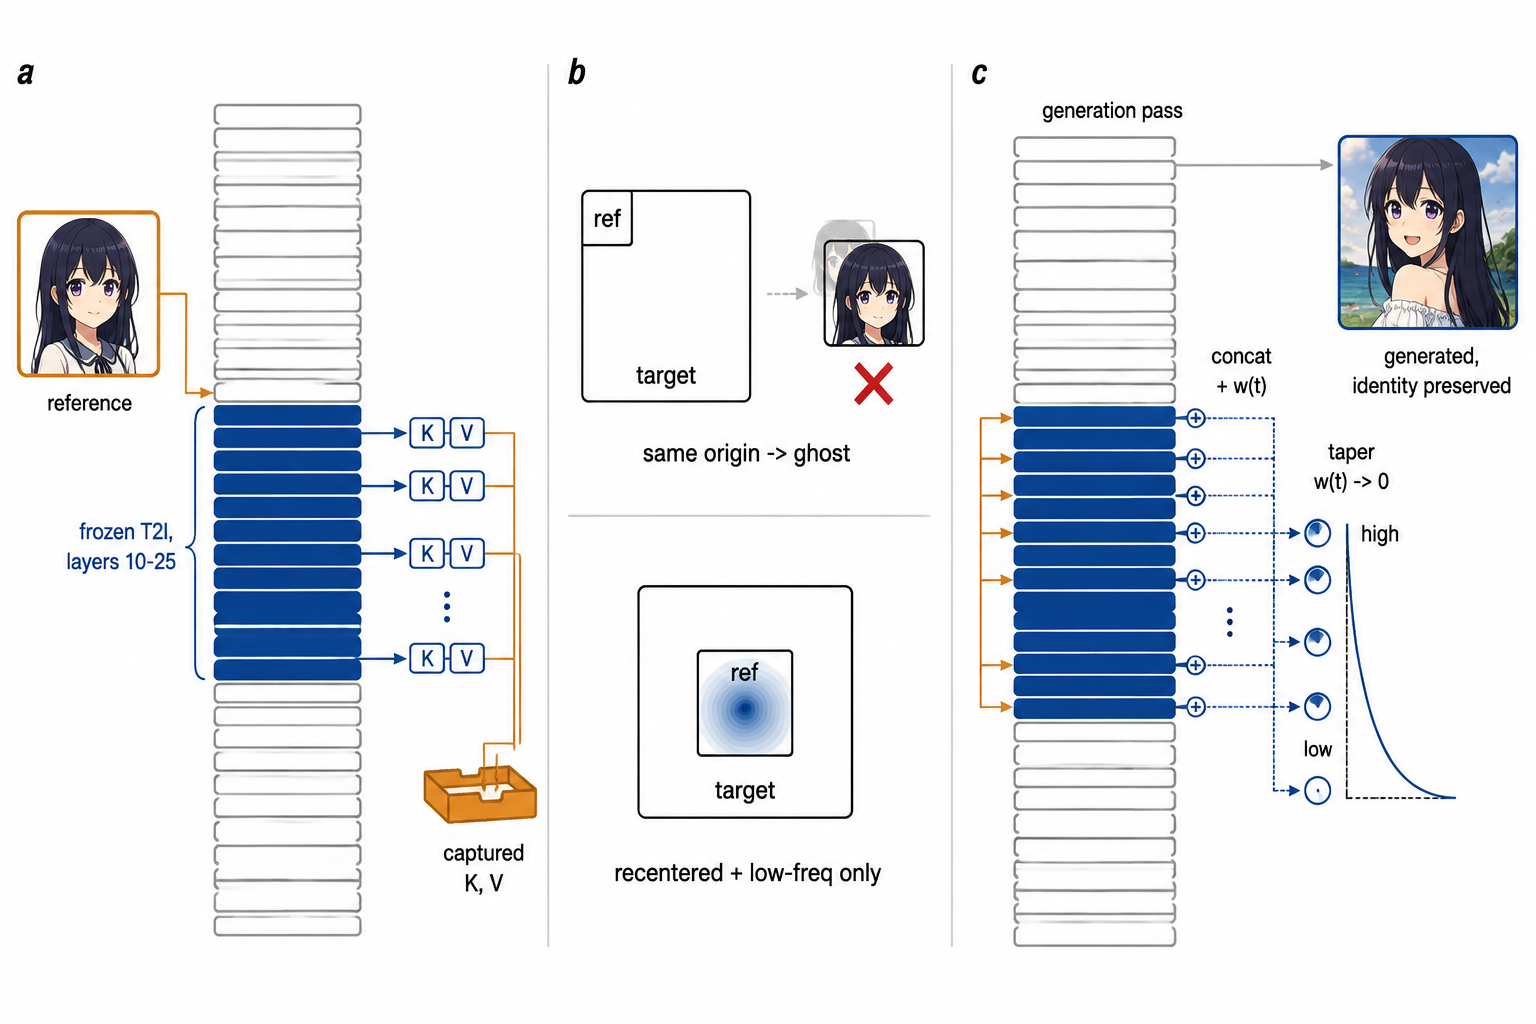
\includegraphics[width=0.85\textwidth]{figs/mechanism_diagram_kv_injection.png}
  \caption{The ref-KV injection mechanism (Method). (a)
  Capture pass: reference K/V stored from a layer band. (b) Naive
  same-origin injection ghosts; the fix re-centers RoPE and keeps only
  low-frequency channels. (c) Generation pass: captured K/V concatenated
  in, scaled by a taper $w(t)$. Conceptual illustration, no quantitative
  data encoded.}
  \label{fig:mechanism}
\end{figure*}

\section{Experiments: Training-Free Mechanism}\label{sec:results-tf}

\subsection{Evaluation protocol}\label{sec:protocol}

CCIP (anime-domain character similarity, SAME threshold 0.178) is a fast
pre-filter only; it is confirmed insensitive to several failure modes
(hair-color changes, gender/hairstyle flips) a downstream VLM judge
catches. We report Gemini 3.1 Pro's \texttt{same\_character: yes/no/partial}
judgment (ref vs.\ generated, ignoring pose/outfit/background) as the
primary identity metric. Held-out and baseline judgments add a second,
independent \texttt{visible\_defect: yes/no} field to the same judge call
(rendering artifacts only -- tiling, duplication, broken anatomy;
explicitly not art-style or pose) and report the \emph{joint} metric,
using an explicit chain-of-thought prompt (the model reasons through each
identity axis and the composition check in prose before emitting JSON).

\subsection{Dev-set ablation (band width $\times$ position gating)}\label{sec:devablation}

10 subjects, 2--4 seeds, random sample, $n{=}20$--$40$, Wilson 95\% CI.
Every row is measured on the same 10 subjects band width and
\texttt{lowfreq\_k} were tuned against -- reported to document the tuning
process; the held-out validation below is the number that matters for
any external claim.

\begin{table}[t]
\centering\small
\begin{tabular}{@{}lrrr@{}}
\toprule
Recipe & $n$ & yes & no (95\% CI) \\
\midrule
\texttt{strip}, band 21--25 (prior default) & 40 & 18\% & 25\% [14,40] \\
\texttt{center}, band 21--25 & 20 & 10\% & 55\% [34,74] \\
\texttt{lowfreq} $k{=}8$, band 21--25 & 20 & 0\% & 30\% [14,52] \\
\texttt{lowfreq} $k{=}8$, band 10--25 & 40 & 58\% & \textbf{0\% [0,9]} \\
\bottomrule
\end{tabular}
\caption{Dev-set band/position ablation (identity-only metric).}
\label{tab:devablation}
\end{table}

\subsection{Held-out validation: the recipe reverses}\label{sec:heldout}

Recipe frozen at \texttt{band=10-25, refpos=lowfreq, lowfreq\_k=8,
sched=taper, w=4.0} \emph{before} running this section. 30 subjects
disjoint from the dev set, 2 seeds, paired against the old default on the
same subjects/seeds, single blind judgment pass.

\begin{table}[t]
\centering\small
\begin{tabular}{@{}lrrrr@{}}
\toprule
Recipe & $n$ & defect & clean-yes & clean-usable \\
\midrule
old (\texttt{strip}) & 60 & 20\% [12,32] & 13\% [7,24] & \textbf{53\% [41,65]} \\
new (\texttt{lowfreq}) & 60 & \textbf{82\% [70,89]} & 8\% [4,18] & 15\% [8,26] \\
\bottomrule
\end{tabular}
\caption{Held-out defect and joint (usable-output) metric. clean-yes = identity=yes \& no defect; clean-usable = identity$\in\{$yes,partial$\}$ \& no defect.}
\label{tab:heldout}
\end{table}

Read in isolation, the marginal identity metric looks like a modest win
for the new recipe (yes: 23\%$\to$40\%) -- exactly the framing the
defect field above was designed to guard against. 79\% of the new
recipe's ``yes'' verdicts also carry a defect flag
(19/24). On usable-output rate the 95\% CIs do not overlap: the
position-free baseline is usable 53\% of the time; the frequency-gated
recipe, 15\%. The defect is a composition failure -- collaged/tiled
sub-images, picture-in-picture insets, duplicated fragments
(Fig.~\ref{fig:holdout}) -- far more frequent than a minor artifact. Both
arms share the same subjects, reference images, and seeds; only the
injection recipe differs, ruling out a data-source confound. The
reversal is CI-decisive on defect rate and clean-usable rate; on strict
identity match alone the CIs overlap (directional, not decisive, at
$n{=}60$/arm). \textbf{Conclusion: \texttt{strip}/band 21--25 is the
recipe this work recommends for deployment}; \texttt{lowfreq}/band
10--25 remains a research direction with a real, unresolved defect mode.

\subsection{Baseline comparison}\label{sec:baseline}

IP-Adapter-SDXL (\texttt{ip-adapter-plus-face\_sdxl\_vit-h}, no per-subject
training, same 30 held-out subjects) is the same-\emph{method}-class
trained-adapter baseline -- its own SDXL backbone, not Z-Image, and never
adapted to the anime domain it is tested on here, so this is a same-class
reference point, not an architecture- or domain-controlled comparison.
\texttt{krea2-identity-edit} (community LoRA on the 12.9B general-domain
Krea-2-Turbo, zero retraining by us) is likewise purpose-trained and
architecturally distinct. Neither baseline is architecture-matched to our
Z-Image backbone; both are the strongest publicly available bars we could
run at zero additional training cost.

\begin{table}[t]
\centering\small
\begin{tabular}{@{}lrrr@{}}
\toprule
Recipe & defect & clean-yes & clean-usable \\
\midrule
IP-Adapter-SDXL & 33\% & 18\% [11,30] & 58\% [46,70] \\
krea2-identity-edit & \textbf{2\% [0,9]} & \textbf{33\% [23,46]} & 58\% [46,70] \\
this work, \texttt{strip} & 20\% [12,32] & 13\% [7,24] & 53\% [41,65] \\
this work, \texttt{lowfreq} & \textbf{82\% [70,89]} & 8\% [4,18] & 15\% [8,26] \\
\bottomrule
\end{tabular}
\caption{Four-arm held-out comparison, $n{=}60$ each.}
\label{tab:baseline}
\end{table}

Restricting to the two general-adapter-class arms (\texttt{strip},
IP-Adapter): both metrics nominally favor IP-Adapter, but every CI
overlaps heavily -- neither ranking is decisive at this sample size. The
defensible claim is \textbf{training-free \texttt{strip} is statistically
indistinguishable from a same-class trained adapter's strict-identity
rate, at zero training cost} -- not that it beats one. That does not
extend to krea2: against \texttt{strip}, krea2 is CI-decisive on defect
rate and clean-yes, but only directional on clean-usable. krea2's
near-elimination of the collage defect fits its mechanism -- a source
latent trained end-to-end as a structured in-context token, unlike raw
K/V concatenated post-hoc into attention pools the frozen model never
expected -- but krea2 also has the \emph{highest} outright-miss rate of
all four arms (40\% vs.\ IP-Adapter's 15\%): most reliable when it
works, most likely to miss outright when it does not. Manual inspection
(Fig.~\ref{fig:baseline}) shows three qualitatively distinct failure
signatures -- \texttt{lowfreq} collages, IP-Adapter garbles hands, krea2
normalizes/drops accessories toward a generic prior rather than
mis-rendering them -- not one mode at three severities. \texttt{lowfreq}
remains decisively worst on both strict metrics despite the highest raw
identity-match rate, reinforcing that
identity-match alone does not reliably rank these methods.

\subsection{No localized handle for the defect}\label{sec:repairs}

If the identity signal were localized, the collage defect should have a
local handle -- a layer, a head, a token, or a denoising phase -- that
suppresses it while sparing identity. We probed four such handles on the
injection mechanism, each against a matched control, and the training
objective of Sec.~\ref{sec:auxloss} is a fifth; none separates the defect
from identity. \emph{(i) Background isolation.} Matting the reference to
a white background (the content-leakage hypothesis) leaves the
composition defect essentially unchanged (combined collage/other rate
$88\%\to80\%$; the residual is a top-left positional artifact class, not
per-reference leakage). \emph{(ii) Head-gating.} Restricting injection to
the top-quarter attention heads by reference affinity does not beat a
random-quarter or bottom-quarter control ($n{=}12$), and the
top-affinity selection is in fact weakest on identity, so the apparent
``fewer heads, cleaner'' effect is injection \emph{count}, not head
selection. \emph{(iii) Outlier-token suppression.} Zeroing high-norm
reference tokens is indistinguishable from a same-count random-drop
control. \emph{(iv) Late-timestep gating.} Withholding injection until
the low-noise phase removes the collage cleanly, but identity collapses
with it (0/5 subjects retain reference-specific identity), because
identity and composition co-form in the early denoising pass. Each
result is individually modest, some at small $n$, but they agree in
direction across four independent injection-side handles plus the
training objective -- the outcome a distributed, composition-entangled
identity predicts and a localized one does not. We do not claim no handle
\emph{can} exist; we report that none of the natural layer-, head-,
token-, timestep-, or objective-level handles we tested works.


\begin{figure*}[t]
  \centering
  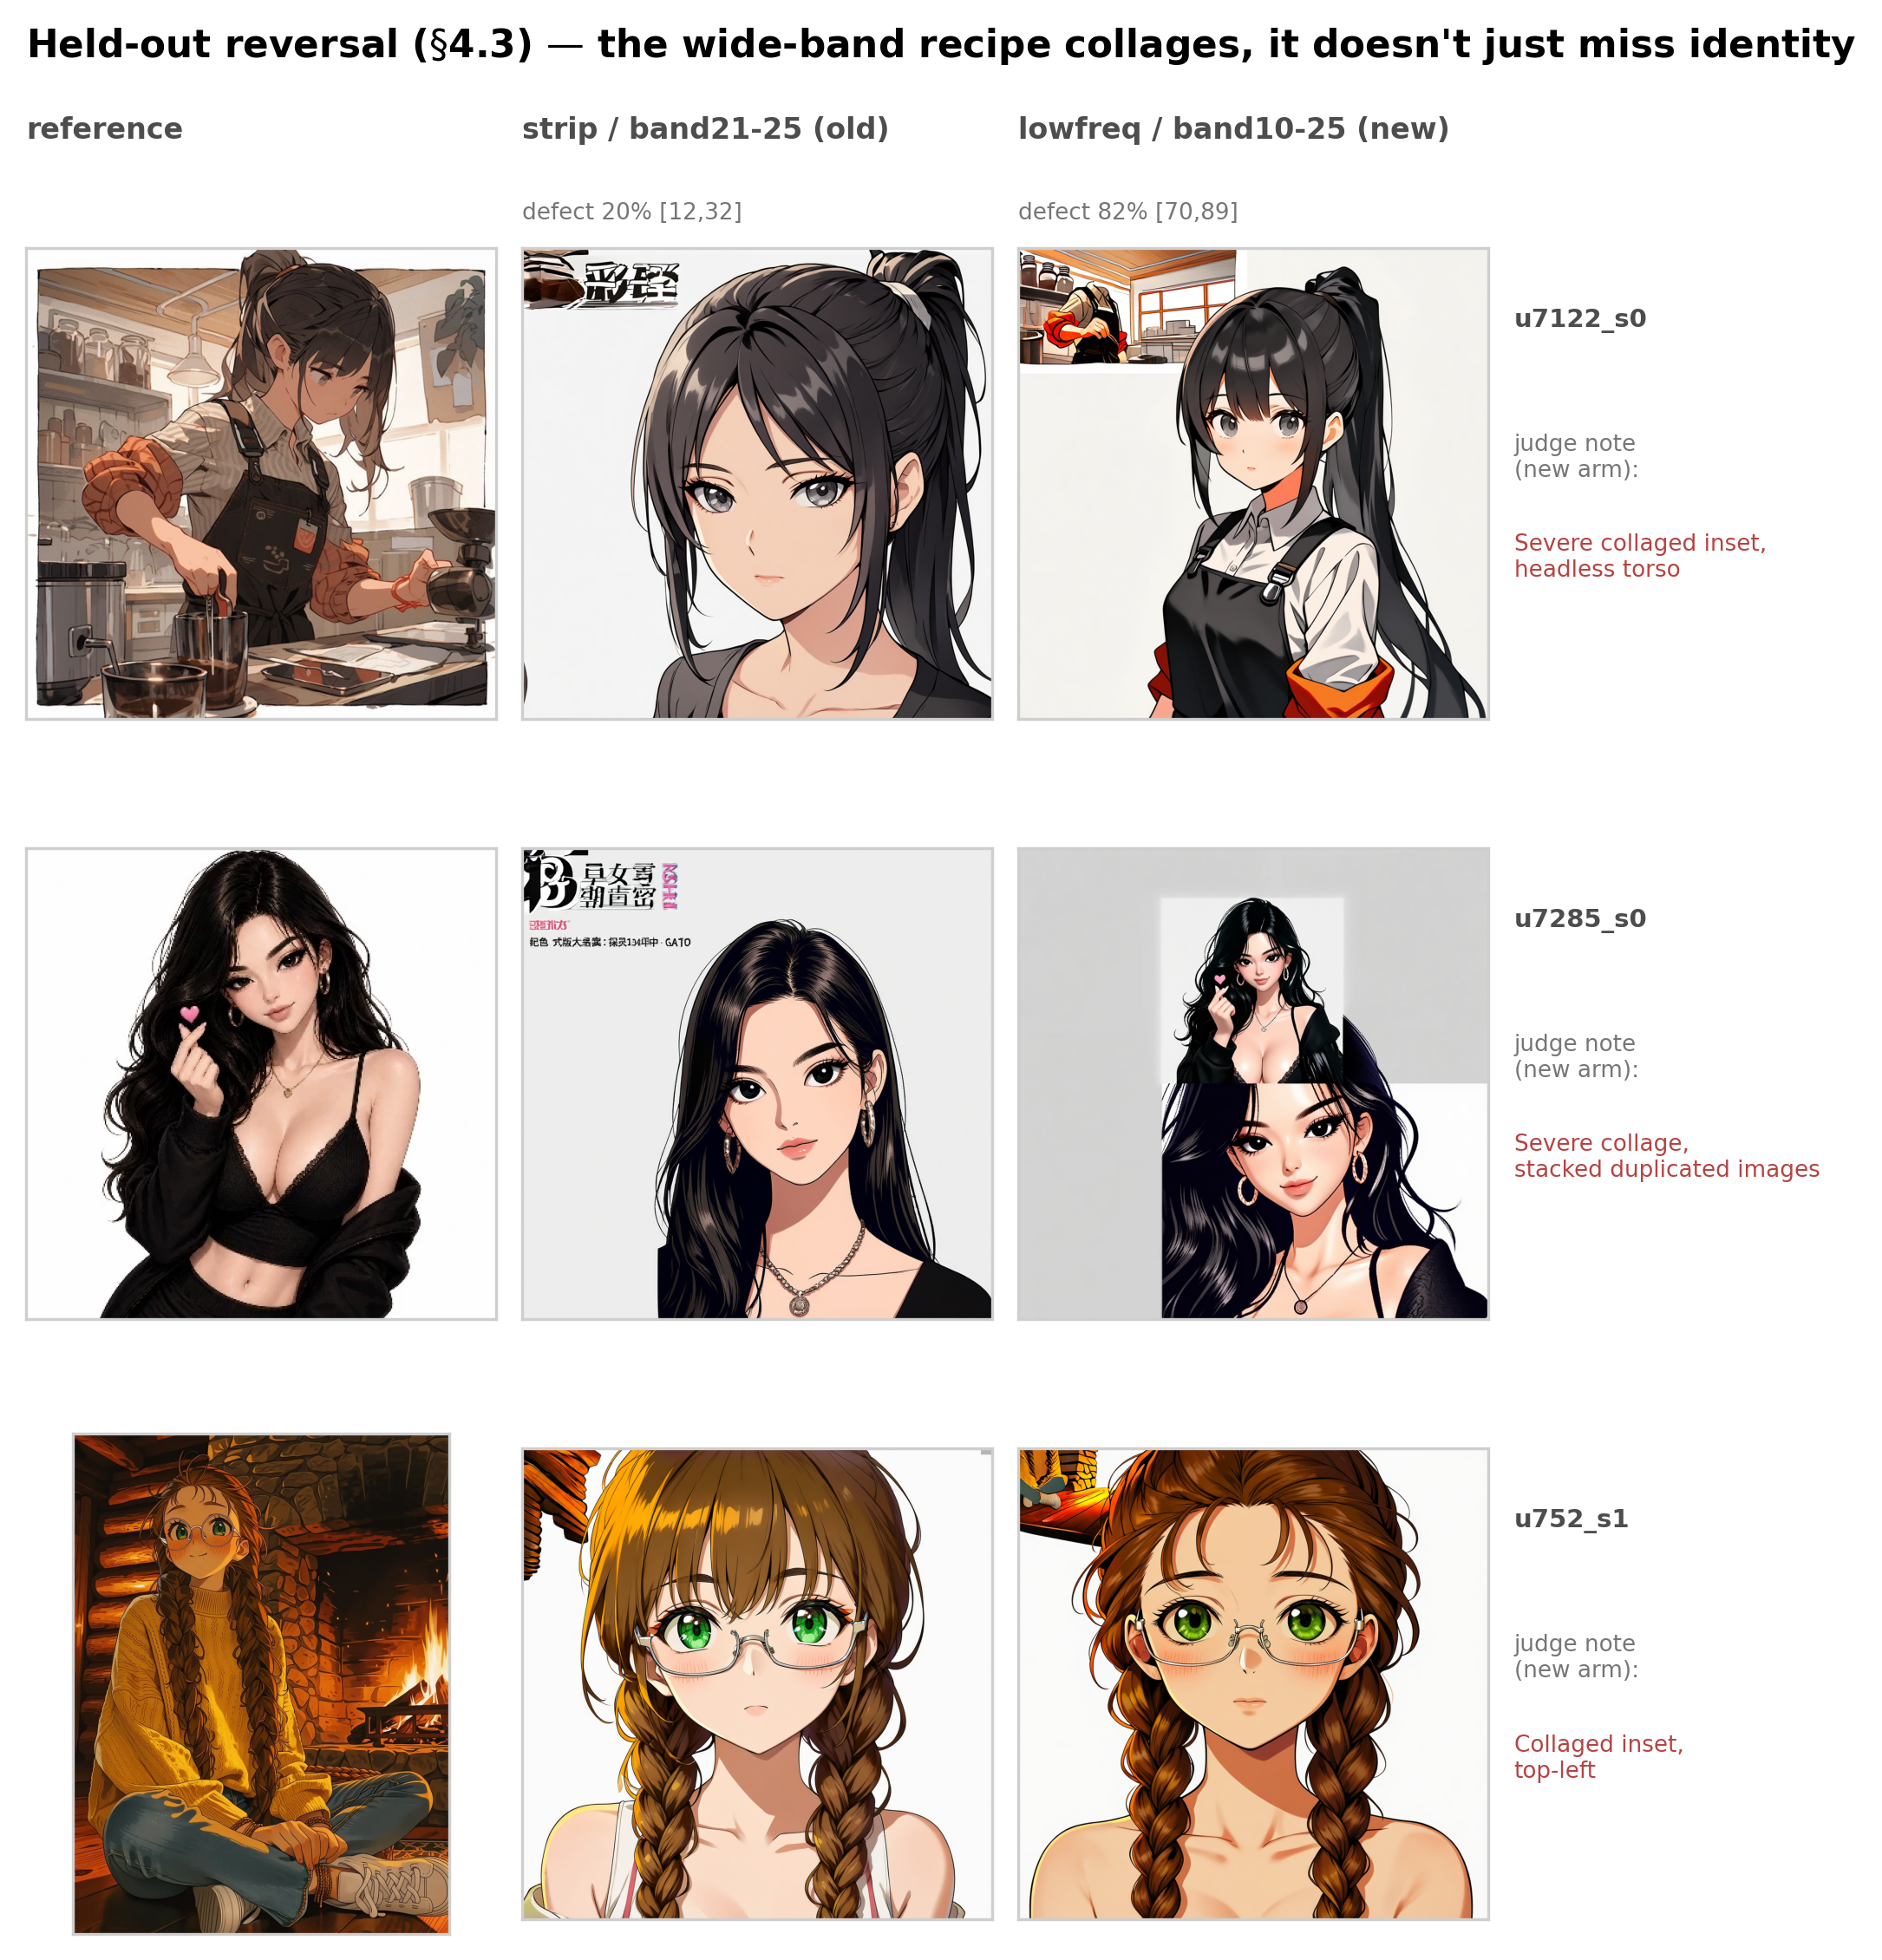
\includegraphics[width=0.85\textwidth]{figs/holdout_reversal_defect_qualcheck.png}
  \caption{Held-out reversal: three subjects,
  \texttt{strip} (old) vs.\ \texttt{lowfreq} (new), same subject/seed. All
  three show \texttt{same\_character=yes} for the new recipe, but a
  collaged/tiled sub-image corrupts the composition -- the failure mode
  behind the 82\% held-out defect rate.}
  \label{fig:holdout}
\end{figure*}

\begin{figure*}[t]
  \centering
  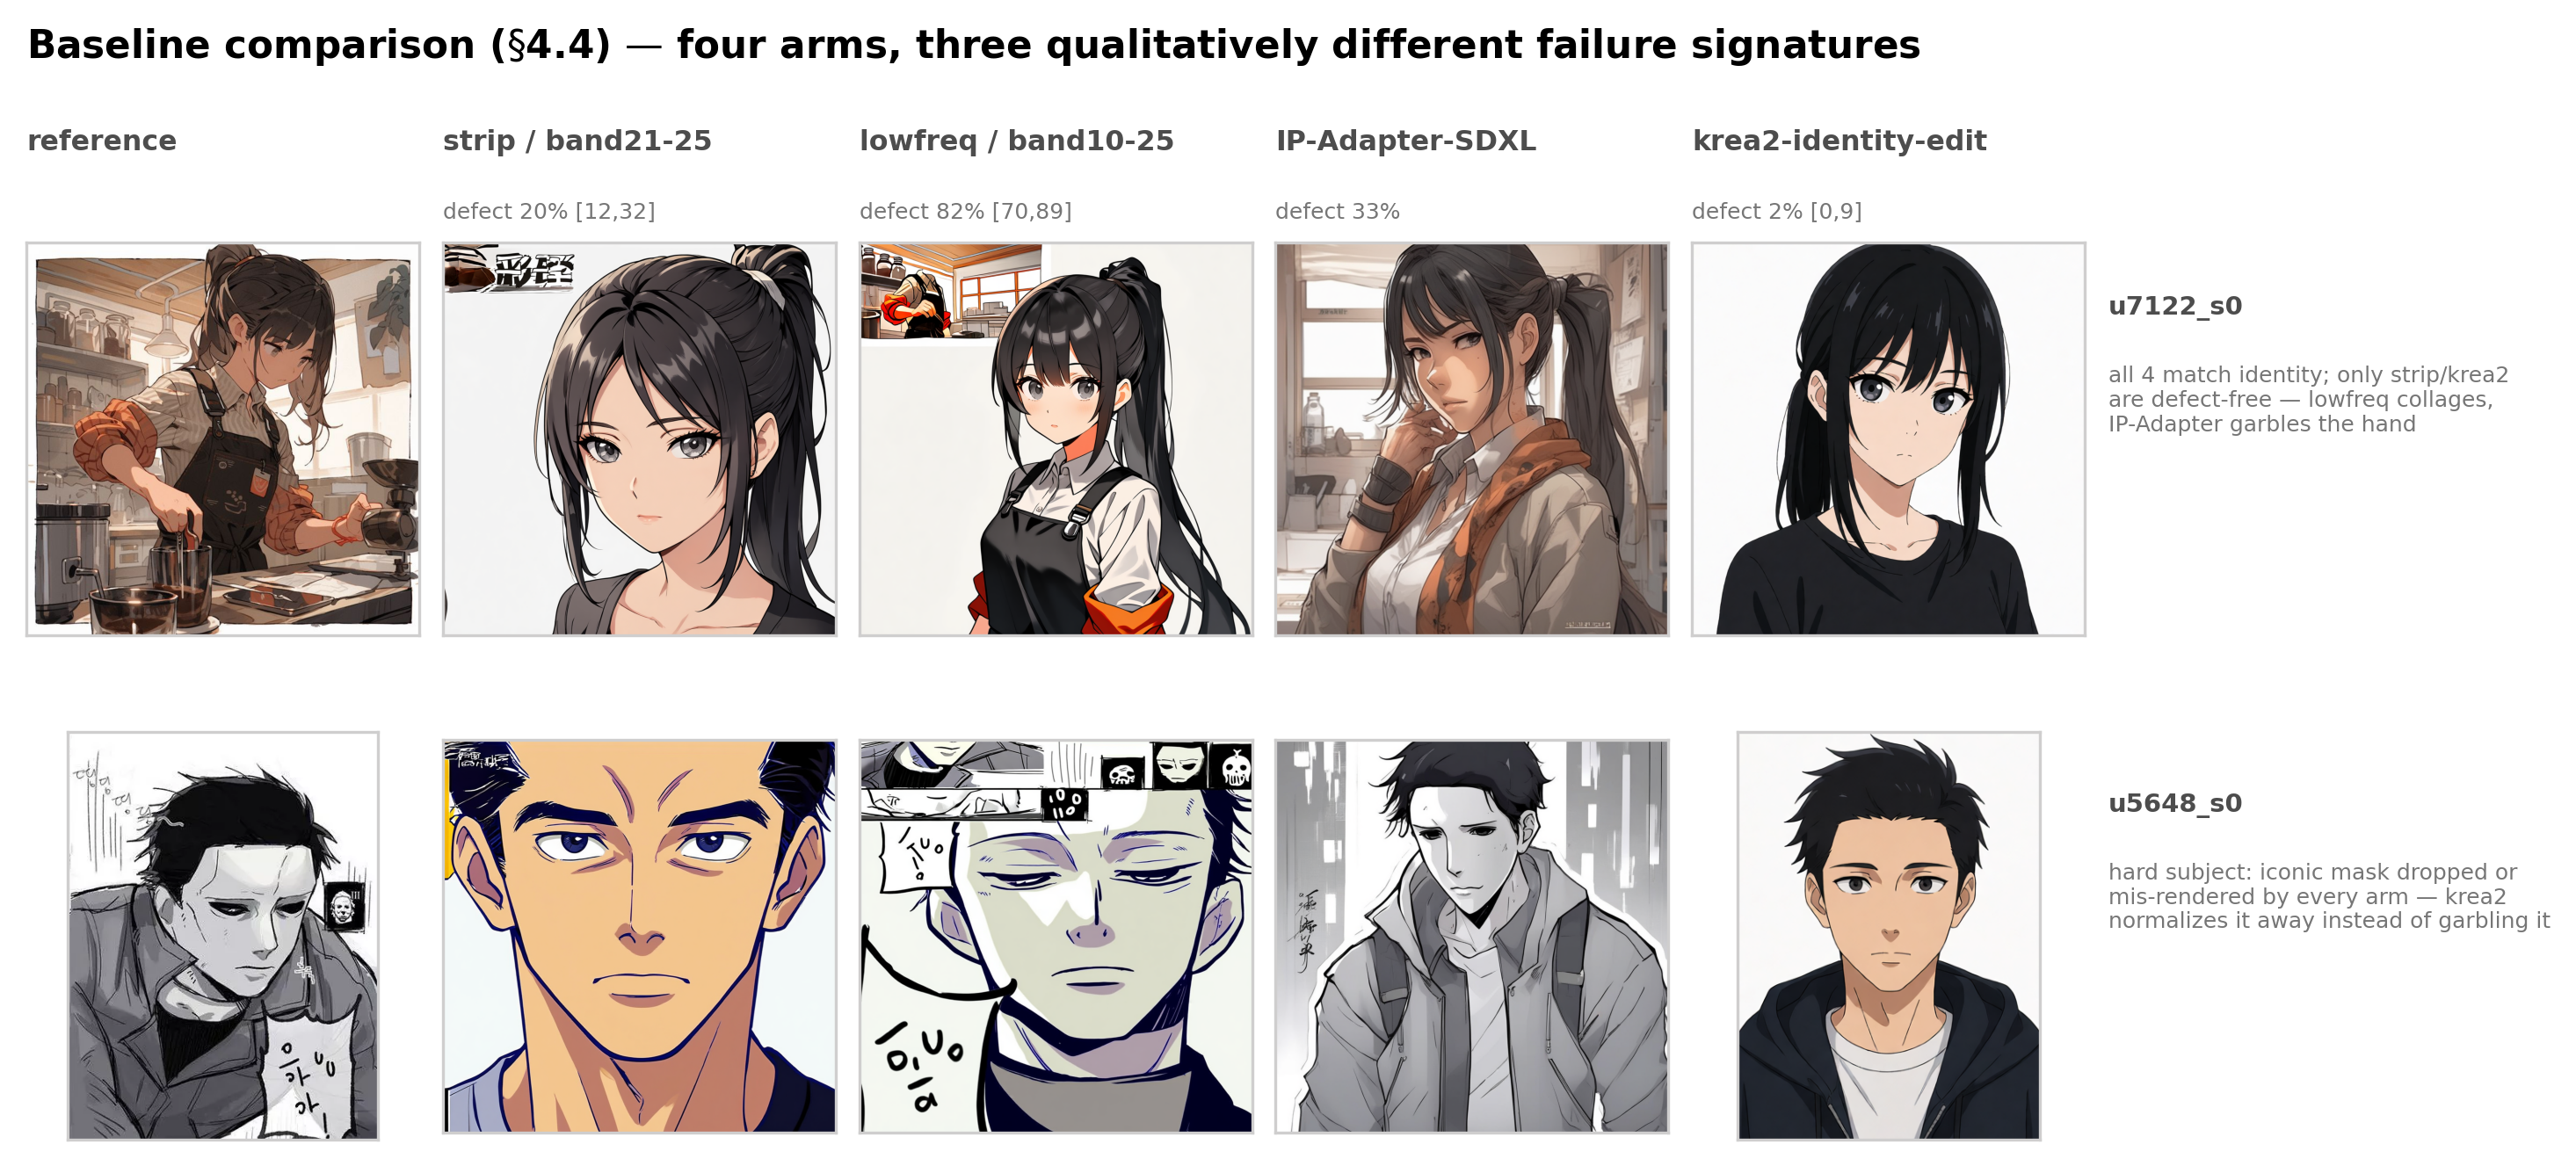
\includegraphics[width=0.85\textwidth]{figs/baseline_comparison_qualcheck.png}
  \caption{Baseline comparison: top (u7122),
  identity matches in all four arms but only \texttt{strip}/krea2 are
  defect-free -- \texttt{lowfreq} collages, IP-Adapter garbles the hand.
  Bottom (u5648), a hard subject every arm misses, but
  differently: \texttt{strip}/IP-Adapter/krea2 normalize the dropped
  accessory, \texttt{lowfreq} also collages -- three distinct failure
  signatures, not one.}
  \label{fig:baseline}
\end{figure*}

\section{Experiments: Training-Light Mechanism}\label{sec:results-tl}

\subsection{Layer-position ablation}\label{sec:bandablation}

Four band-LoRA arms, matched trainable-parameter budget (early 0--15
$r{=}8$; mid 10--25 $r{=}8$, a pre-existing production checkpoint; late
14--29 $r{=}8$; full-depth 0--29 $r{=}4$, rank lowered to stay near the
16-layer arms' 3.93M-parameter budget), 4000 steps, held-out 30-subject
dev set $\times$ 2 seeds ($n{=}60$/arm), same defect-aware judge protocol
as the training-free experiments above. The reused mid checkpoint later
proved \emph{not} protocol-matched to the other arms (different
training-manifest revision; a style prefix in its generation prompts) --
a confound we discovered, quantified, and resolve below. \textbf{Pre-registered decision rule,
locked before the three missing arms were run}: a band counts as
specially favored on identity-match only if its clean-yes point estimate
is highest \emph{and} its 95\% CI does not overlap the worst arm's.

\begin{table}[t]
\centering\small
\begin{tabular}{@{}lrrr@{}}
\toprule
Arm & clean-yes & defect & clean-usable \\
\midrule
early 0--15 ($r{=}8$) & 15.0\% [8,26] & 8.3\% [4,18] & 45.0\% [33,58] \\
mid 10--25 ($r{=}8$)$^\dagger$ & 21.7\% [13,34] & \textbf{3.3\% [1,11]} & 55.0\% [42,67] \\
late 14--29 ($r{=}8$) & 21.7\% [13,34] & 18.3\% [11,30] & 46.7\% [35,59] \\
full-depth ($r{=}4$) & 23.3\% [14,35] & \textbf{28.3\% [19,41]} & 43.3\% [32,56] \\
\bottomrule
\end{tabular}
\caption{Band-position ablation on the first dev set, $n{=}60$/arm,
Wilson 95\% CI. $^\dagger$The mid row was measured under a non-shared
protocol; a protocol-matched re-run yields defect 30.0\% [20,43] (see
text).}
\label{tab:bandablation}
\end{table}

\textbf{Primary metric result: null, replicated.} All four clean-yes
CIs overlap (highest, full-depth, 23.3\% [14,35]; lowest, early, 15.0\%
[8,26]) -- under the pre-registered rule, band position is \emph{not}
specially favored for identity-match. The a priori hypothesis (``10--25
is the identity band'') fails on its own designed test. A full re-run
of all four checkpoints on a second, disjoint held-out 30-subject set
(zero retraining, identical judge) reproduces the null: clean-yes
18.3--25.0\%, all CIs overlapping. Identity capacity is depth-uniform
in every cell we measured.

\textbf{Secondary observation, refuted by our own audit.} On the first
set, defect rates appeared to form a CI-decisive gradient
(3.3\%$\to$8.3\%$\to$18.3\%$\to$28.3\%; subject-clustered mid 6.7\%
[0,17] vs.\ full-depth 43.3\% [27,60], non-overlapping). Three audits
then killed it. \emph{(i) Cross-set replication fails}: on the second
set the interior ranking inverts (late becomes best, 8.3\%; mid
second-worst, 20.0\%) and mid-vs.-full-depth clustered CIs overlap
(36.7\% [20,53] vs.\ 46.7\% [30,63]). \emph{(ii) The mid arm was
double-confounded}: a completed 2$\times$2 factorial (checkpoint
$\times$ prompt-prefix, $n{=}60$/cell) closes the attribution instead
of bounding it -- the prefix effect is checkpoint-specific, not
portable ($+13.3$pp within run\_mix1, $+0$pp within run\_mix2), and the
only clustered-CI-disjoint marginal is the checkpoint swap at
prefix-on ($+26.7$pp); clean-yes stays flat across all four cells
(16.7--21.7\%). \emph{(iii) A confound-free mid} (same recipe,
matched manifest, no prefix) scores 30.0\% [20,43] defect on the
\emph{original} set -- clustered 53.3\% [37,70], disjoint from the
confounded 6.7\% [0,17] -- and is cross-set stable (26.7\% on the
second set). Under a uniform protocol every arm sits in an 8--30\%
defect band with no stable position ordering; full-depth is numerically
worst on both sets but never CI-separated from mid. A seeded random
audit of judge flags (10 of 17 full-depth flags, all mid flags,
negative controls) additionally found only 30--70\% of flags
correspond to real damage depending on severity threshold (zero false
negatives on controls) -- raw judge rates overstate severe-defect
rates. What survives is the null: layer position determines neither
identity capacity nor, as far as our evidence goes, defect rate.

\subsection{Does an identity-supervised objective separate the
defect?}\label{sec:auxloss}

If the collage defect were a training deficiency rather than a
structural entanglement, adding an explicit identity signal to the
objective should buy identity without the defect. We test this directly.
From a config-matched MSE-only baseline (band 10--25, $r{=}8$, mix3
manifest, seed 0, 1500 steps), two arms add one auxiliary loss and
nothing else: a decode-space CCIP identity loss (weight 0.05) and a
perceptual loss (weight 0.1). Evaluated on the full held-out
30-subject set $\times$ 2 seeds ($n{=}60$/arm) with the same
defect-aware judge, neither helps (Table~\ref{tab:auxloss}): both leave
clean-yes at or below the MSE baseline while \emph{raising} the defect
rate -- the identity-loss arm to 26.7\% and the perceptual arm to
40.7\%, against the baseline's 13.3\%. The most direct training-side
repair moves the tradeoff the wrong way rather than dissolving it. This
is the fifth matched-control repair, and the only training-side one, to
trade identity for coherence rather than separate them -- consistent
with a defect entangled with identity, not one caused by weak
supervision.

\begin{table}[t]
\centering\small
\begin{tabular}{@{}lrr@{}}
\toprule
Arm ($n{=}60$) & clean-yes & defect \\
\midrule
MSE baseline & \textbf{16.7\% [9,28]} & \textbf{13.3\% [7,24]} \\
+ CCIP identity loss & 15.0\% [8,26] & 26.7\% [17,39] \\
+ perceptual loss & 10.2\% [5,20] & 40.7\% [29,53] \\
\bottomrule
\end{tabular}
\caption{Auxiliary-loss pilot, held-out $n{=}60$/arm, Wilson 95\% CI. An
explicit identity (CCIP) or perceptual objective does not reduce the
composition defect; both raise it without improving identity match.}
\label{tab:auxloss}
\end{table}


\begin{figure*}[t]
  \centering
  
\includegraphics[width=0.56\textwidth]{figs/band_ablation_defect_qualcheck.png}
  \caption{Band-position qualitative check: mid 10--25 vs.\ full-depth
  0--29, same subject/seed. All three
  full-depth cells are judge-flagged defective; inspection confirms
  genuine anatomical breaks absent in the matched mid-band generation.}
  \label{fig:bandablation}
\end{figure*}

\section{Limitations}\label{sec:limits}

\texttt{lowfreq} (band 10--25) is \textbf{not production-ready}: 82\%
held-out defect rate collapses usable-output to 15\% despite a higher
raw identity-match rate. \emph{Why} is partially decomposed: a
position-information-free variant at the same widened band is
statistically as defective (75\% vs.\ 71\% on a dev probe), ruling out
position-encoding precision as the driver -- injecting reference
content into layers 10--20 at all is what destabilizes; no cheap fix
emerged.
Geometric attributes (face/eye shape) remain a residual failure for the
recommended (\texttt{strip}) recipe even where composition is clean
(45\% partial rate). The frequency-gating sweet spot ($k{=}8$) and band
width (10--25) were tuned on a 10-subject dev set using a metric later
shown insufficient; re-tuning on a fresh, disjoint probe set is future
work, as are AnimeAdapter and FreeGraftor/UNO baselines (no public
weights / gated dependency).

For the training-light mechanism, $n{=}60$ is 30 subjects $\times$ 2
seeds, not 60 independent draws; headline comparisons therefore carry
subject-clustered CIs alongside per-image ones. The defect-gradient
audit chain (different-family cross-judge, seeded random flag audit,
cross-set replication, confound-free re-run) is reported in the results
section; each step independently weakened the gradient before the
ensemble refuted it, and the first warning was visible early -- GPT-5.5
had already failed to reproduce the gradient's magnitude. Attribution
of the confounded mid arm's advantage is now closed, not bounded: the
completed checkpoint$\times$prompt-prefix factorial shows the prefix
effect is checkpoint-specific, not portable ($+13.3$pp within
run\_mix1, $+0$pp within run\_mix2), and the only clustered-CI-disjoint
marginal (checkpoint at prefix-on, $+26.7$pp) still overlaps at
prefix-off -- inseparable there from ordinary run-to-run training
variance. Absolute numbers are modest
regardless of arm: 51.7--55.0\% clean-usable / ${\sim}20$\% clean-yes
is not state-of-the-art accuracy in either line of this work; the
contribution is the anatomy of the identity signal and the evaluation
methodology, not benchmark accuracy. All experiments ran on a single
141GB-class GPU (LoRA training ${\sim}4$--$6.5$h per arm; generation
${\sim}35$\,min per 60 images).

\paragraph{Scope of the distributed-identity claim.} The
non-localization evidence is bounded by the handles we tested (continuous
layer bands, reference-affinity head subsets, high-norm token sets,
timestep gates); a finer or compositional handle could in principle
localize identity, and we claim only that these natural handles do not.
The two mechanisms are independent as \emph{interventions} but share
evaluation \emph{instruments} (one judge, one CCIP stack, one anime data
family), so their agreement is corroborative, not fully independent. The
cross-architecture selectivity signature is correlational on $n{=}2$
models -- a within-model RoPE-$\theta$ test was inconclusive by
construction -- so we offer it as a diagnostic, not a cause. All evidence
is single-domain (anime) on one main model; whether the account transfers
to photographic identity or other DiT families is open, and contrary
locality findings in prior work may reflect that setting difference.

\section{Conclusion}\label{sec:conclusion}

We activated a frozen, pure-T2I anime diffusion transformer as a
one-shot reference-conditioned identity generator two independent, cheap
ways -- zero-training attention KV injection and a 0.06\%-parameter
band-LoRA -- each statistically tied with a same-class trained baseline
on identity (\texttt{strip} with IP-Adapter at zero training cost; the
band-LoRA with krea2 at 0.06\% of its parameters), reported as ties, not
wins, with a shuffled-reference control confirming the conditioning is
genuinely reference-driven. Using these mechanisms as probes, our central
finding is an anatomy: the one-shot identity signal in this frozen DiT is
\emph{distributed and composition-entangled}. Within the handles we could
test it is not localized -- to any layer band (a null replicated across
two held-out subject sets and concurring across both mechanisms), head
subset, or denoising phase -- and the collage defect is entangled with
identity rather than separable from it, as five matched-control repairs
each confirm by trading identity for coherence rather than removing the
defect. A peaked-versus-diffuse attention-selectivity signature, offered
as a cross-architecture diagnostic, further separates a model that
transfers structured identity from one that transfers only mean color.
Two measurement reversals along the way show that identity-match-only,
single-set evaluation is systematically optimistic for this class of
method. The composition-collapse mode is characterized but unfixed, and
geometric-attribute fidelity remains a residual failure even for the
recommended recipe.


\bibliography{references}

\end{document}
